\documentclass[12pt]{ctexart}
\usepackage[utf8]{inputenc}
\usepackage{geometry}
\geometry{left=1in,top=2.25in}
% \setlength{\parindent}{1em}
\setlength{\parskip}{1em}
\usepackage{xeCJK}    % 加载 xeCJK 宏包以支持中文
\usepackage{graphicx}
\usepackage{subfigure}
\usepackage{booktabs} % 导入booktabs包,用于创建三线表格
\usepackage{multirow}
\usepackage{amsmath}
\usepackage{hyperref}
\usepackage{amsfonts}
\usepackage{indentfirst} % 加载 indentfirst 宏包以使首段缩进
\usepackage{enumitem}
\setlist[enumerate]{label=(\arabic*)}
\usepackage{titlesec}
% \titlespacing{\section}{0pt}{\parskip}{-\parskip}
% \titleformat{\section}[block]{\normalfont\Large\bfseries}{\thesection}{1em}{}[\hspace{\parindent}] % 设置每个section第一段不缩进
% 设置绿色的引用和链接
\hypersetup{
    colorlinks=true,
    citecolor=green,
    linkcolor=green,
    filecolor=magenta,      
    urlcolor=cyan,
}

% 在目录中恢复原来的颜色
\makeatletter
\AtBeginDocument{%
  \pretocmd{\tableofcontents}{\hypersetup{citecolor=black,linkcolor=black}}{}{}%
}
\makeatother

% 设置 tocdepth 为 2,目录仅显示到二级标题
\setcounter{tocdepth}{3}

\usepackage{tocloft}

% 设置目录条目的行间距
\setlength{\cftbeforesecskip}{2.5ex} % 这里的 1ex 是你可以调整的行间距



\title{
\Huge{\textbf{商业分析报告}}\\
\Large{\textbf{BUSNESS ANALYSIS REPORT}}\\
\vspace{8mm}
% 
\includegraphics[width=5cm]{Images/logo.png}\\
% \vspace{25mm}
}
\author{\textbf{Task 3} \\
\textbf{AUTHOR: 杨唯茜 Estella}\\
% \textbf{Student Number: 202119293}\\
% Supervisors: \\
}
\date{DATE.vr1: 2024/10/18  \\
      % DATE.vr2: 
      }




\pagestyle{empty}

\begin{document}
\newgeometry{right=1in,left=1in,top=1.5in,bottom=0.75in}
\maketitle
\thispagestyle{empty} % 去页数标记

\vspace{5mm}





\newpage
\clearpage
\thispagestyle{empty}
\newgeometry{right=0.75in,left=0.75in,top=1in,bottom=1in}
\thispagestyle{empty} % 去页数标记
\begin{titlepage}
{
\clearpage
\thispagestyle{empty}
  % 在目录之前设置颜色
  \color{black}
  \tableofcontents
}
\end{titlepage}
\newpage


\pagestyle{plain} 

\clearpage % 插入空白页
\pagenumbering{arabic}

\section{电商平台的直播带货}

\subsection{经济的上风口}
\begin{quote}
    \textit{“In live commerce, the lines between performance and purchase blur, as we witness the artistry of curation coming alive before our eyes.”} \\
    \raggedleft \textit{- Anna Wintour, a Vogue editor}
\end{quote}

Vogue Business在今年6月发布的一篇报告\cite{1}中称:直播开启电子商务新时代,97\% 的 Z 世代消费者表示社交媒体是他们购物灵感的首要来源,根据欧睿国际的数据,到 2022 年,该市场将产生超过 1500 亿美元的收入,且预计未来两年内,直播将占电子商务销售额的 20\%。 

\begin{figure}[htbp!]
    \begin{minipage}[t]{0.48\textwidth}
        \centering
        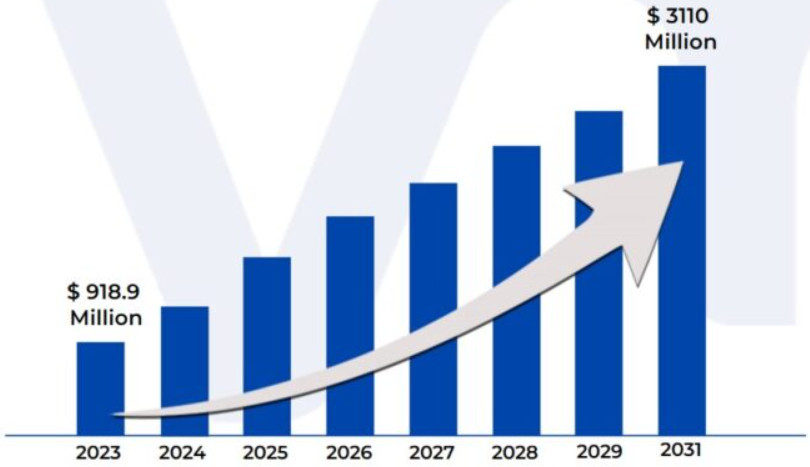
\includegraphics[width=\textwidth]{Images/1.png}
        \caption{2024-2031(估计)全球直播电商市场\cite{2}}
        \label{global}
    \end{minipage}
    \hfill
    \begin{minipage}[t]{0.48\textwidth}
        \centering
        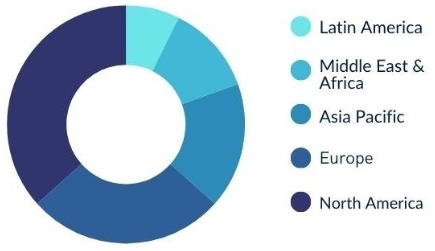
\includegraphics[width=\textwidth]{Images/2.png}
        \caption{2023年全球电商市场地区占比 \cite{3}}
        \label{region}
    \end{minipage}
\end{figure}

如图(\ref{global})所示,这个市场一片向好,2024到2031年的年复合增长率预计为16.45\%;北美地区,就像图(\ref{region})所展示的,占据的最大的市场份额\cite{1}。直播是电子商务和娱乐的结合体,它能实时展示产品,摆脱了强迫性的广告,转向更真实的代言,这个模式在中国市场已大获成功\cite{1}。

\begin{figure}[htbp!]
    \centering
    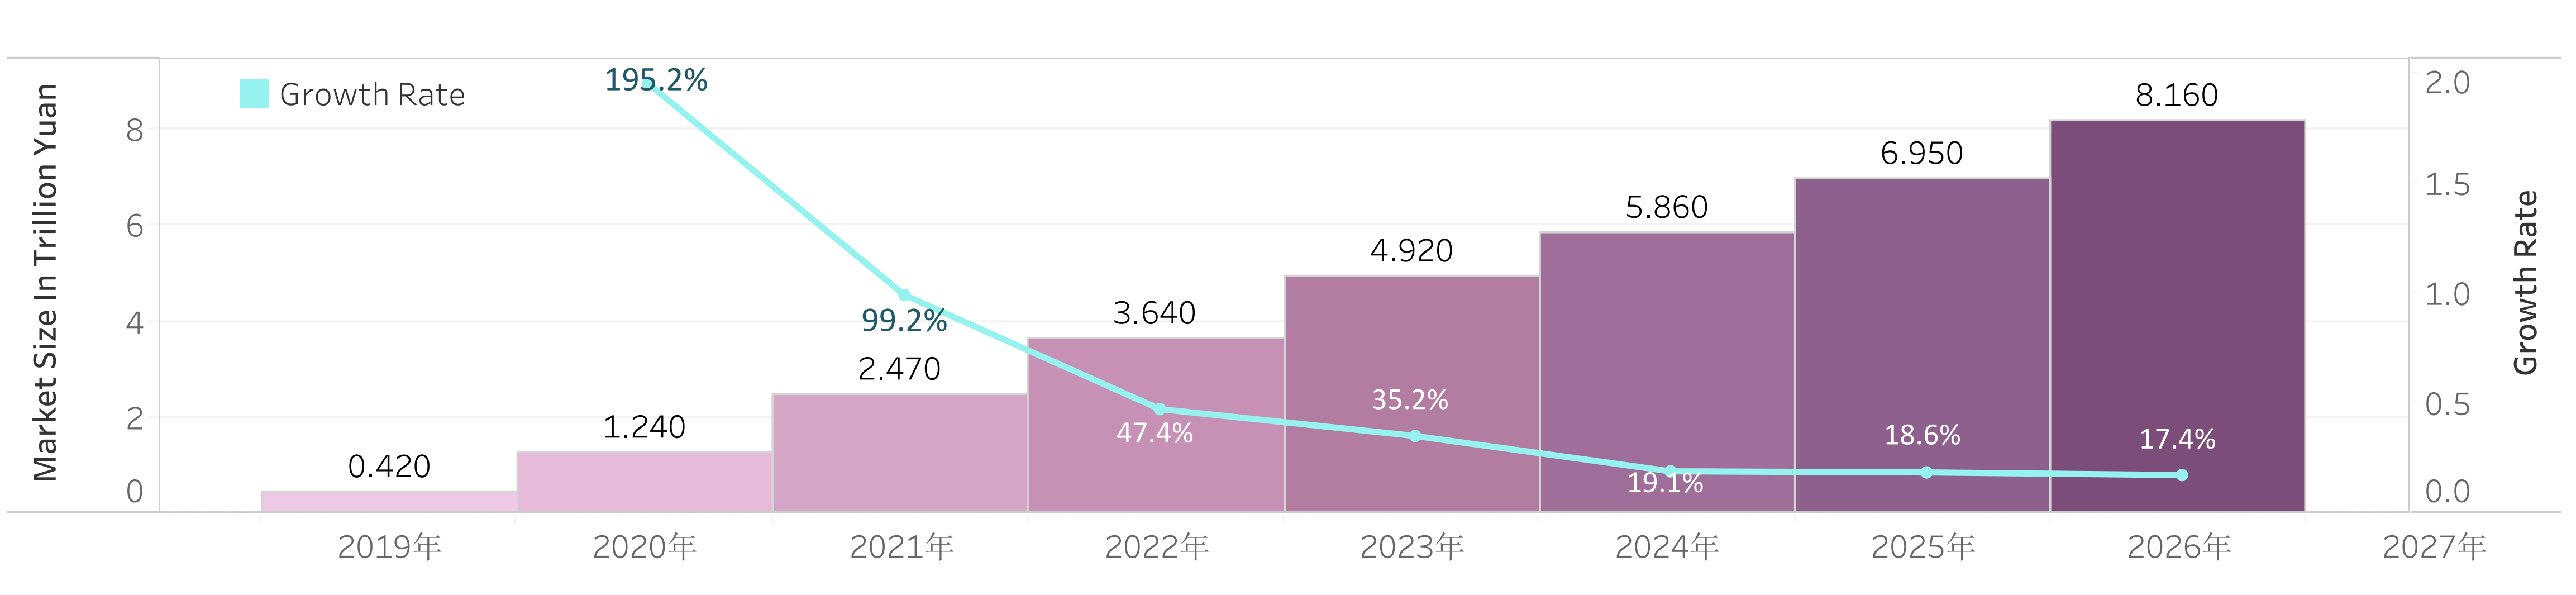
\includegraphics[width=1\textwidth]{Images/3.png}
    \caption{2019-2026(估计)中国直播电商市场规模(单位:万亿元) \cite{3}}
    \label{china}
\end{figure}





\subsection{Amazon Live 销售数据整理复盘}

Amazon作为电商巨头,自然没理由缺席这个新兴的盛宴\footnote{本文作者搜索了很久Amazon Live的销售数据,但一直没有办法找到。这个章节就能查找到的排名、评价讨论。}。2016年Amazon推出Amazon Live,自此进入直播电商市场,不过由于其开始地比其他平台晚,且本身不以直播作为业务之一,因此并不占领先地位。2022年的一次调研显示,Facebook Live、Instagram Live是最受消费者欢迎的两大直播购物平台之一,而Amazon Live和TikTok Live共同位居第三(图(\ref{popu}))。

\begin{figure}[htbp!]
    \centering
    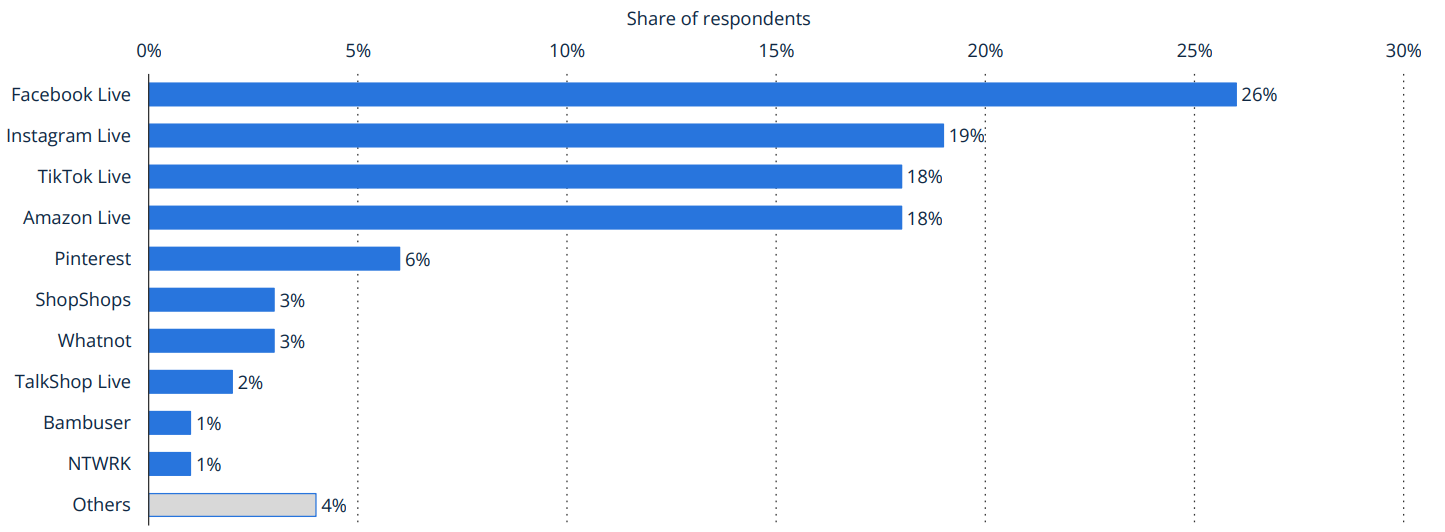
\includegraphics[width=0.9\textwidth]{Images/4.png}
    \caption{2022年美国地区最受欢迎的直播购物平台排名 \cite{4}}
    \label{popu}
\end{figure}

Amazon Live 在推出后收到了不少好评,如Pattern的品牌合作伙伴 Owlet在Amazon Live上推出了关于婴儿床、电脑主机和 Owlet 自营产品的直播活动,结果显示,在一周的销售中Owlet 的销量出现了约 9-16\%的激增,其中,Owlet 袜子监视器的畅销排名提高了令人震惊的 70\%、相机提高了 69\%,但二者的组合销售下降了12\% \cite{5},总的效果非常不错。此外,Pattern另一个品牌合作伙伴 Coravin也尝试过Amazon的直播活动,他们在Cyber Monday 12 天后)发布了葡萄酒保存系统的演示视频,促销活动从2019年12 月 14 日到 12 月 21 日结束,观看次数达到 15,000 次,开播点击率达到了12.5\%,他们的分析师说,Pattern在这期间的表现超越了Black Friday \cite{6}。

不过,并不是所有关于Amazon Live的评价都是正向的,如eMarketer在2021年发布的报告中对新兴直播电商平台NTWRK在四次购物节的直播活动中收获了“平均1000万次观看”、“累计25万名活跃买家”的数据表现做出了称赞,但认为Amazon Live的卖家数过少\cite{7}。Marketplace Pulse在2022年甚至给出了比较尖锐的评价,称“Amazon Live is Embarrassing”,他们说,在 2021 年 Prime Day 期间,它拥有30,000-70,000 名活跃观众,同年11月模仿Twitch、YouTube等重建了 Amazon.com/Live 体验,但Amazon Live 在平常一天最多只有不到一千名活跃观众\cite{8}。

但就图(\ref{popu})和“1亿2022 Prime Day观看量”\cite{5},Marketplace Pulse过于负面,并不可取。

\subsection{受欢迎的产品与直播时间段}
McKinsey \& Company在2022年分地区对直播购物产品受欢迎程度做了调研,见图(\ref{cate}),在美国、拉丁美洲、欧洲,销量最高的都是服装类产品,且都有约40\%的人购入这一品类,而在中国,最畅销的则是日常用品,服装类则屈居第二。这个结果也是可以预见的,不妨打开你手机上的直播平台,主播们总是在展示品牌服装、美妆类产品或卷纸、毛巾等生活类用品。\footnote{本文作者查找了很久,同样没有找到Amazon Live具体受欢迎的时间段等数据,只能找到一点论坛讨论。}

\begin{figure}[htbp!]
    \centering
    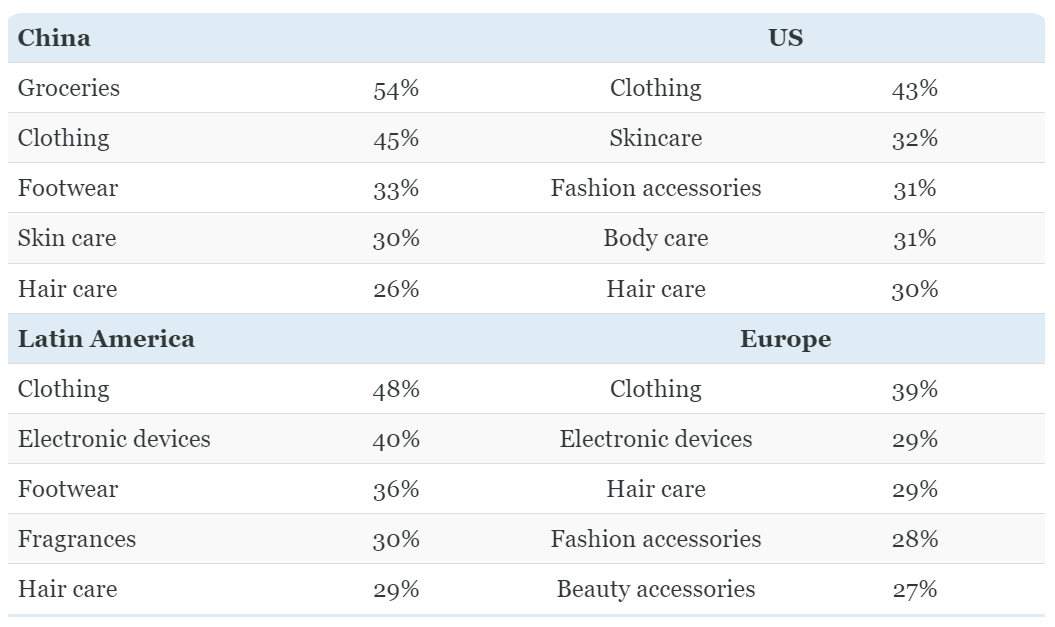
\includegraphics[width=0.8\textwidth]{Images/5.png}
    \caption{2022年通过直播电商购买的前五大品类及其用户比例 \cite{7}}
    \label{cate}
\end{figure}


\subsection{直播带货的成功因素和改进空间}
直播带货这一新兴模式在中国市场已经取得了巨大的成功,在全球视角上来看,也获益匪浅。Fit Small Business在今年1月发布的关于直播电商的32个数据的报告\cite{5}中提到,使用直播商务策略的公司的转化率高达 30\%,比平均转化率高出 10 倍;对一些直播购物活动而言,转化率最高可达 70\%(平均约9\%,仍比普通活动2.5\%-3\%的转化率高出三倍不止);且近一半参与直播活动的零售商预测未来两年将实现 10\%-50\% 的强劲增长,另有 16\% 预计增长将超过 50\%。

\begin{figure}[htbp!]
    \centering
    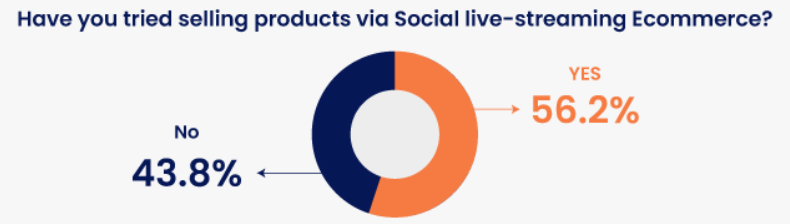
\includegraphics[width=0.7\textwidth]{Images/6.png}
    \caption{2023年GoodFilms 对企业参与直播销售活动的调研结果(N=671) \cite{7}}
    \label{cate}
\end{figure}

为什么零售商们对直播带货的快速增长这么确信呢?或者说,藏在这个模式背后的成功因素到底是什么呢?不妨从以下几个角度来分析:
\begin{itemize}
    \item \textbf{即时互动与信任建立.} \\
    美国 (42\%) 和欧洲 (38\%) 频繁参与直播的购物者表示,他们选择直播购物的首要原因是他们认为直播是一种娱乐 (或“好玩”的) \cite{10},就像之前提到的那样,直播带货方式是将娱乐与销售融合在了一起。加拿大零售商ALDO在2021年举办了一场直播后,发现参与度增加了308\%,且在直播后的五天内,网站访问量达到了17,000次\cite{11},以让消费者看到真实效果的形式大幅提升了品牌信任度和回访率。这都是“直播”直接带来的好处。
    \item \textbf{现场促销与优惠的紧迫感.} \\
    \cite{11}中提到了“FOMO”效应,即“害怕错过”的心理,因为在一对多的直播购物场景中,品牌通常会举办直播视频购物活动,面对大量观众,某一特定产品的销售可能只会持续十多分钟,以TikTok为例,用户可以在直播中看到其他人购买或将商品加入购物车的行为,随着当前折扣商品倒计时滴答减少,这似乎在催促着他们也需要赶紧做出举措。这跟购物节的“限时秒杀”的效果是类似的,但是由于其是现场促销的特性,通常没有那么强烈的冲动导向,并不会引起反感情绪。当直播观看成为消费者主导的行为,也没有理由再怪罪广告了。
    \item \textbf{视觉冲击与有效的产品展示.} \\
    实时进行产品演示可以让买家了解产品的用途和功能,从而帮助他们更好地理解产品,甚至可以让观众“抢先一睹”即将推出的产品,在上架之前就创造需求\cite{12}。还可以展示多种产品变体和选项,并实时回答买家对产品颜色、尺寸、适合度和用途等方面的疑问,这种视觉冲击将使消费者们“真实”体验“线下购物”,将虚拟带至现实。梅西百货的社交策略高级总监Sara Holmgren表示,他们发现直播购物的顾客是最具粘性的客户之一\cite{11}。
    \item \textbf{社交属性与口碑传播.} \\
    在线购物的一大缺陷是缺乏与产品的实际互动,虽然AR和VR技术有所改善,但其并不普及且“触感”有限\cite{12},直播使购物者们能够与销售主播互动、与观众互动,这种近乎真实的感官购物体验是无可替代的。“直播总不能有假吧?”,很多人都会这么想,“眼见即真”,由于其直播的形式,消费者还可以方便地将直播间地址转发给自己的好友,达成自发的品牌口碑传播,使用Emplifi直播购物解决方案的零售商,平均订单价值提高了36\% \cite{12}。
    \item \textbf{名人效应与KOL推荐助力.} \\
    近年,网红营销变得越来越重要,网红营销行业规模预计到 2023 年将增长到约 211 亿美元\cite{13},他们可以培养人们对产品的信心。名人和KOL拥有大量追随者,他们的推荐会迅速传播,且他们通常具备较强的内容创作能力,能够制作有趣且吸引人的直播内容,提升观众的观看体验。Amazon在2017年推出过一个Influencer Program,今年8月增加了“Creator Stars”分层组件,激励KOL发布视频\cite{14}。还记得中国的薇娅和李佳琪吗?直播王李佳琪曾以五分钟卖出 15,000 支口红而闻名\cite{15},他们的直播间在“双十一”前后总是人满为患。
\end{itemize}

而对于Amazon Live 而言,其成功因素还有其强大生态系统的依托、先进技术的分析支持。

\begin{figure}[htbp!]
    \begin{minipage}[t]{0.47\textwidth}
        \centering
        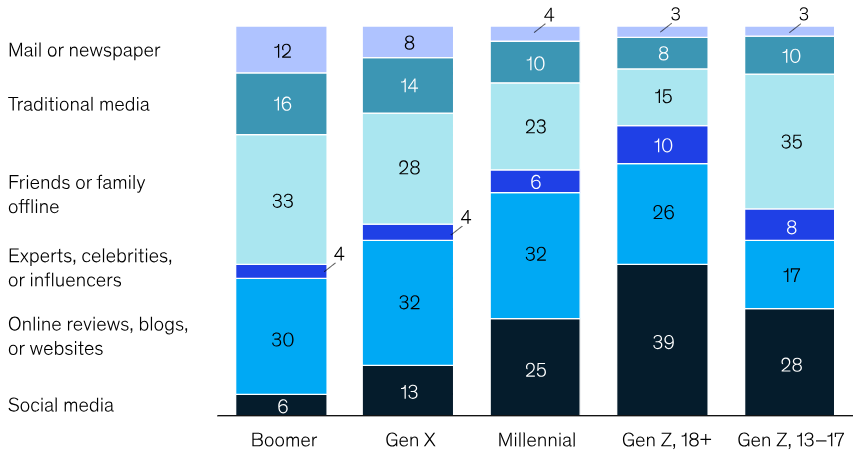
\includegraphics[width=\textwidth]{Images/7.png}
        \caption{各世代受推荐产品或品牌影响来源\cite{10}}
        \label{global}
    \end{minipage}
    \hfill
    \begin{minipage}[t]{0.505\textwidth}
        \centering
        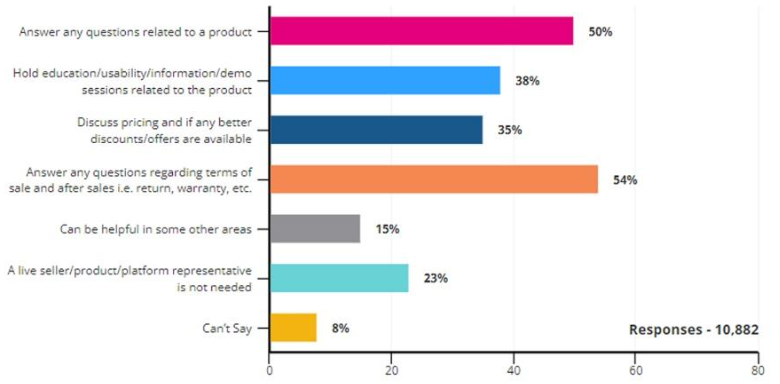
\includegraphics[width=\textwidth]{Images/8.png}
        \caption{直播购物中受到来自主播、平台的帮助 \cite{20}}
        \label{region}
    \end{minipage}
\end{figure}

虽然直播带货已经在中国外的地区逐渐小有成就,但要想达到中国市场的效果,还需持续的策略改进和平台与卖家的共同努力。那么对Amazon Live还有哪些改进空间呢?

从上面的用户行为统计与反馈结果,结合各个地区、平台表现,作出以下改进建议:
\begin{itemize}
    \item \textbf{增强互动性并提升直播质量.} \\
    Amazon Live并不是一个独立平台,而是寄托于Amazon购物平台中的一个部分,可以通过增加实时互动功能,如观众的提问与回答、投票等、打赏或付费弹幕(Twitch、Bilibili等直播平台都有使用)等,增强用户的参与感。目前Amazon Live的直播质量相较于其他直播平台并不是十分令人满意,需要确保主播对产品具备深度了解,并能够清晰展示产品的优势与使用场景,从而增强用户信任感和购买决策的信心,当然,这需要平台与主播共同努力。
    
    \item \textbf{定期举办促销活动并利用其他平台辅助宣传.}\\
    定期推出促销活动(这里说的不仅仅是Black Friday、Cyber Monday、Prime Day等购物节或节假日,而还有独属直播带货的活动)以其独有性吸引观众参与直播。同时建议通过整合外部社交平台(如Instagram、YouTube等)进行联动宣传,利用这些平台的用户基础和影响力来提高Amazon Live活动的曝光率,从而扩大直播的受众群体。
    
    \textcolor{blue}{关于这一点,本文作者有一些拙见:}实际上,Amazon已经收购了Twitch这一最大、最受欢迎(当然,中国地区除外)的直播平台,为什么不将其利用起来呢?既然Amazon Live是一个附属的平台,那么其实可以将Amazon Live整合到Twitch中,可以首先推出针对领头游戏博主的激励活动,与他们合作(就像Bilibili中百大博主们经常接广告这样,但是由于平台的性质,这里的产品最好为电子类商品),利用他们的粉丝基础将消费者引至购物平台。让各个品牌入住Twitch内部的Amazon Live,再将这部分发展扩大。但是,这样做确实也有一定风险,本文作者并不认为Amazon Live上直播可以与Twitch火热的游戏直播抗衡。
    
    \item \textbf{多样化内容创作并建立社群.} \\
    不应将内容局限于产品展示,Amazon Live可以拓展到更多类型的内容分类,比如生活方式分享、使用技巧教程、品牌故事等,来吸引更广泛的受众,这里需要博主们主动制作更多、更新的内容,平台可以做的更多的是设置针对某种内容的创作激励计划。此外,鼓励主播与观众建立长期互动的社区,实际上,中国地区已经有很多分享直播购物折扣、优惠劵抢购活动的社群(一般以微信、QQ等社交媒体为介),其他地区可以使用Whatapp、Discord等。
    
    \item \textbf{优化Amazon Live Creator软件.} \\
    这一点的提出是因为Amazon Live Creator的下载评分虽然在Google Play上有4.3/5.0分,但在Apple Store中只有2.8/5.0分,论坛上也褒贬不一。下面是一些截图:

    \begin{figure}[htbp!]
        \centering
        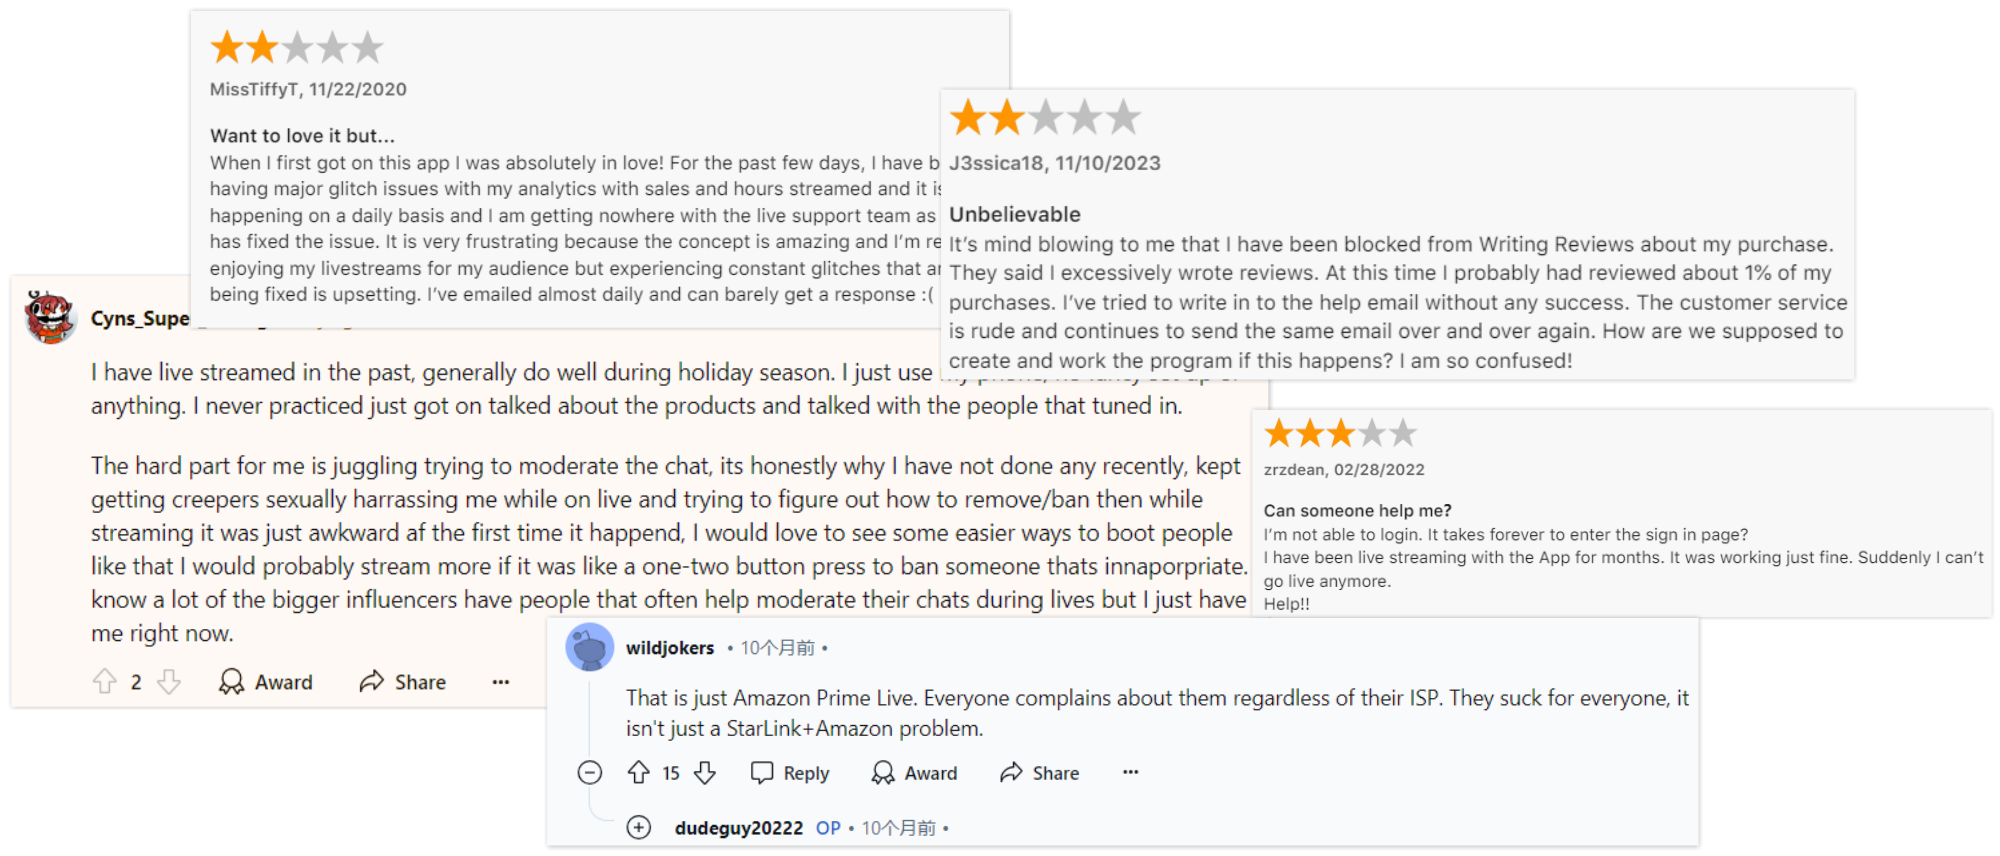
\includegraphics[width=0.95\textwidth]{Images/9.png}
        \caption{一些Apple Store、Reddit上截取的用户关于Amazon Live的评价}
        \label{comment}
    \end{figure}
    
    因此需要进一步改进Amazon Live Creator软件,使其更易于使用并且提供更丰富的功能,如账户兼容登录(可以用谷歌账号等登录)、用户管理工具(Reddit上有人提到性骚扰的问题)、直播效果数据追踪等,帮助创作者更好地理解观众的需求与喜好。同时增强软件的兼容性,优化不同设备上的使用体验,让创作者可以随时随地高效地制作和发布。
    
\end{itemize}

\section{新兴的模式}

\subsection{直播电商与传统电商的异同}
数字零售格局正在经历动态转型,直播购物正成为与传统电子商务并驾齐驱的一股强大力量\cite{16},这两种电商模式有什么异同呢?不妨先从最直接的购物流程说起。

\begin{figure}[htbp!]
    \centering
    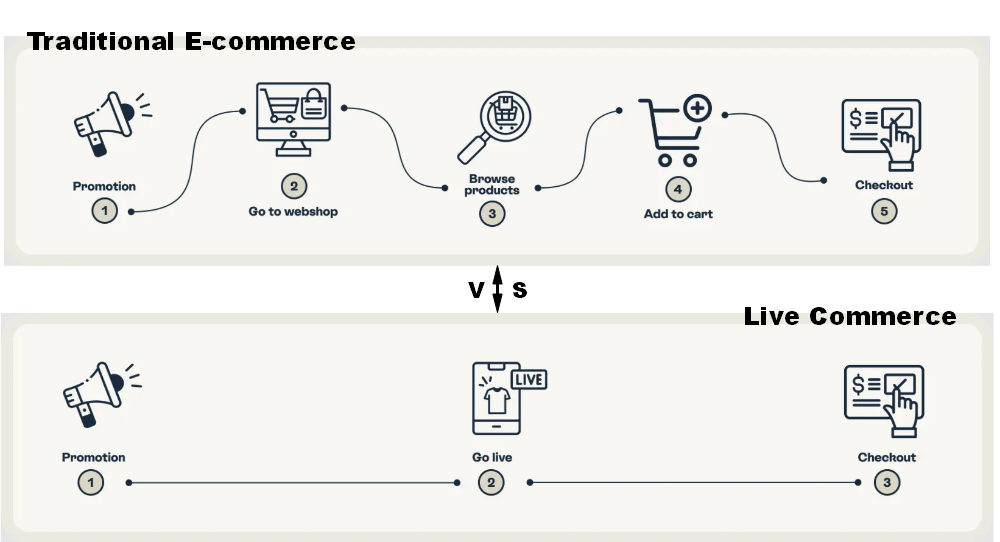
\includegraphics[width=0.8\textwidth]{Images/10.png}
    \caption{传统电子商务用户购物流程与直播电商用户购物流程对比图\cite{16}}
    \label{flow}
\end{figure}

图(\ref{flow})是两种模式的购物流程,可以发现,后者比前者精简了许多步骤,创造了一个顺畅的流程使观众可以从直播中无缝过渡到购买行为,这实际上去掉了冗余步骤中的不确定因素。谁知道消费者会不会懒得搜索网站,或者将商品一直抛弃在购物车直到下架或自动清除呢?

如果用更“专业”的术语来衡量两种模式的话,\cite{16}给出了一个比较完善的表格(图(\ref{index}))。

\begin{figure}[htbp!]
    \centering
    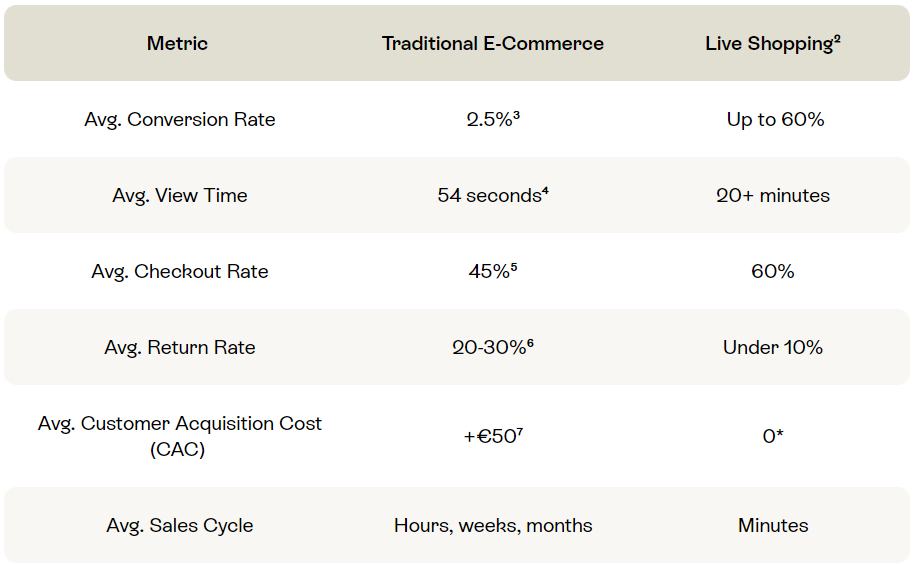
\includegraphics[width=0.7\textwidth]{Images/11.png}
    \caption{传统电商和直播电商模式的关键指标对比\cite{16}}
    \label{index}
\end{figure}

下面分几个层面对两种模式进行对比分析。

\subsubsection{市场定位层面}
两者在市场定位上各有侧重。直播电商主要通过即时的互动和娱乐性内容吸引消费者,定位为一种“边看边买”的购物体验。品牌和商家会选择通过直播快速推送限时优惠、独家折扣,以吸引那些追求即时满足感的消费者。尤其是在年轻一代中,直播电商凭借其娱乐性,俨然成为了一种社交化购物体验。如下图(\ref{interest_us})所示,18-34岁的青年中有约20\%的人都参与过直播购物,虽然这一数据本身不高,但相比于其他年龄段的10\%及以下已经算可观。

\begin{figure}[htbp!]
    \centering
    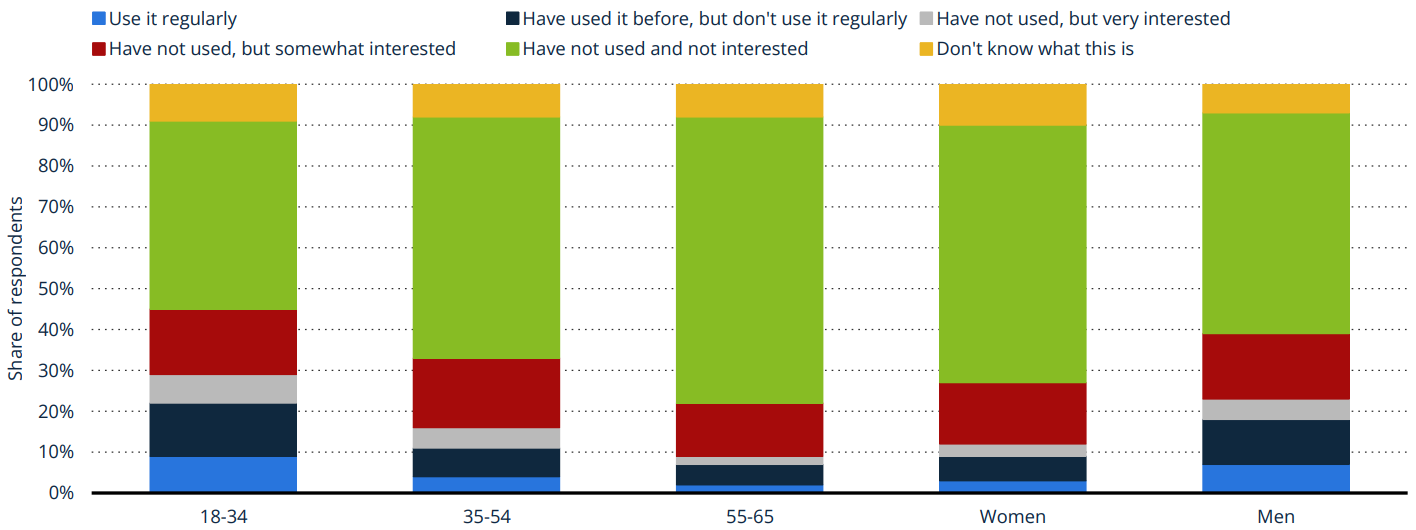
\includegraphics[width=0.85\textwidth]{Images/12.png}
    \caption{2023年美国地区直播/视频电商的感兴趣情况(以性别和年龄段分类)\cite{4}}
    \label{interest_us}
\end{figure}

但在某些地区,年龄分布则呈较均匀的状态,55岁以上的人也没有与年轻人不同(图(\ref{interest_tw}))。

\begin{figure}[htbp!]
    \centering
    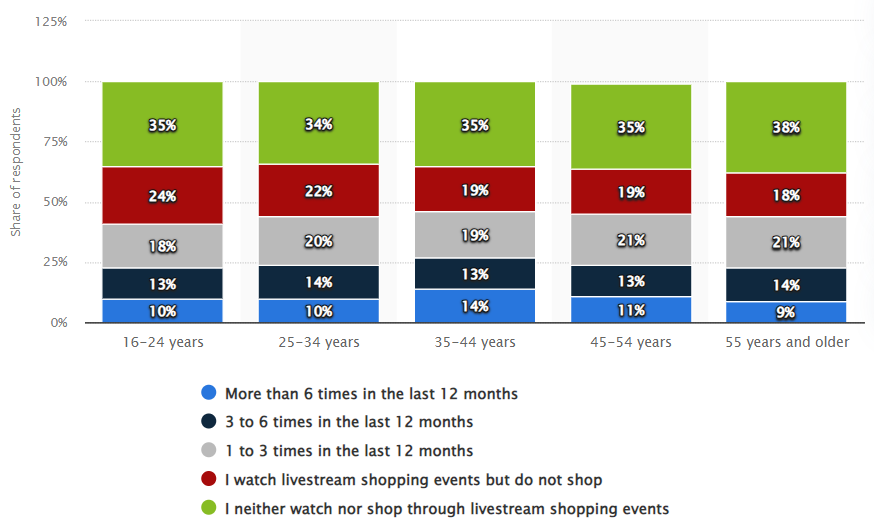
\includegraphics[width=0.93\textwidth]{Images/13.png}
    \caption{2024年5月中国台湾地区通过直播电商购物的频率(以年龄段分类)\cite{17}}
    \label{interest_tw}
\end{figure}

相比之下,传统电商则更专注于“长尾市场”,强调产品的广泛性和选择的多样化。其市场定位更倾向于满足用户的长期需求,例如某些特定产品或大批量的商品。各大平台通过优化用户的搜索体验和提供详细的商品信息,吸引那些以理性购物、价格对比为主的用户群体。传统电商依赖数据分析和算法推荐,为消费者提供个性化的推荐,但缺乏直播那样的互动性。传统电商的用户年龄段分布则比较对称,以中青年人为主(如图(\ref{us_mobile})和图(\ref{all_mobile})移动设备购物情况所示)。

\begin{figure}[htbp!]
    \begin{minipage}[t]{0.31\textwidth}
        \centering
        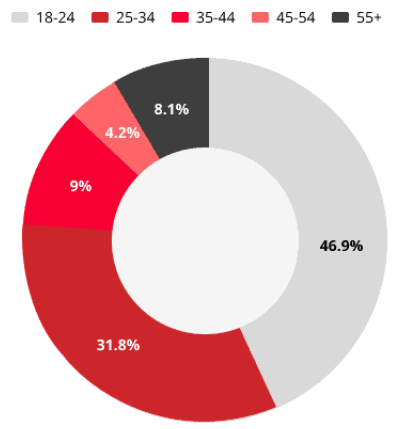
\includegraphics[width=\textwidth]{Images/14.png}
        \caption{2023年美国电商购物者的移动用户群体\cite{18}}
        \label{us_mobile}
    \end{minipage}
    \hfill
    \begin{minipage}[t]{0.667\textwidth}
        \centering
        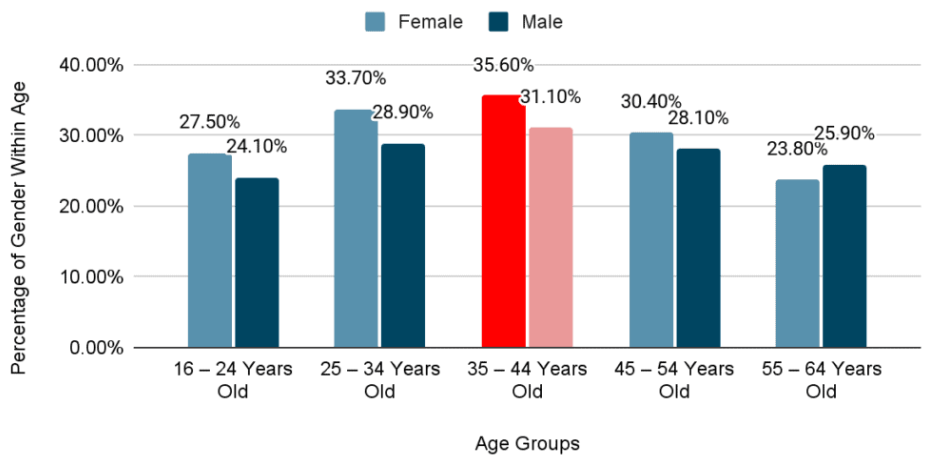
\includegraphics[width=\textwidth]{Images/15.png}
        \caption{2024年各年龄段每周通过移动设备线上购物的百分比 \cite{19}}
        \label{all_mobile}
    \end{minipage}
\end{figure}

\subsubsection{用户体验层面}

在用户体验层面,直播电商依靠互动、即时性和娱乐性来吸引用户。通过实时的产品展示,消费者能够更直观地看到商品的使用效果,并通过直播间的即时提问,得到商家或主播的快速反馈。这种购物模式高度依赖主播的个人魅力和现场氛围。直播不只是产品介绍,更像是一场“秀”,如果主播能够带动直播间氛围,那么用户体验的上限是无限的。

\begin{figure}[htbp!]
    \centering
    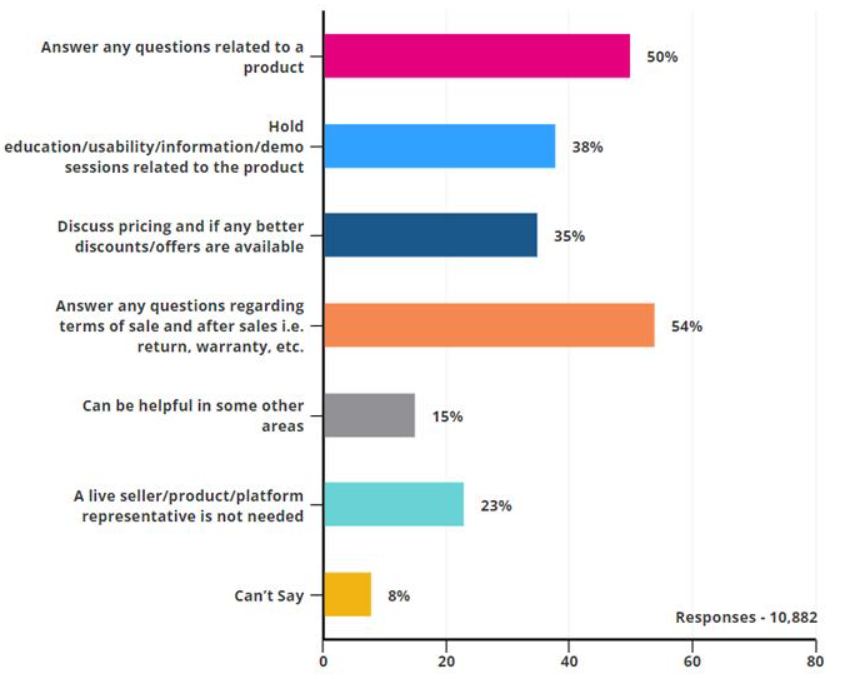
\includegraphics[width=0.75\textwidth]{Images/16.png}
    \caption{2023年印度地区消费者心中直播购物能为他们带来的优点\cite{20}}
    \label{interest_india}
\end{figure}

由图(\ref{interest_india})可以看出,“互动”是直播购物最吸引消费者的原因,他们认为自己能够通过与主播互动直接得到自己想了解的问题的答案,而不是盲目地浏览产品介绍或购物评论。

相比之下,传统电商的用户体验则更强调理性化与自主性。消费者在浏览商品时有更多时间进行研究、比价,用户的购物决策更多依赖于详细的产品描述、用户评价和评分。虽然传统电商也提供推荐系统,但与直播的即时互动不同,推荐算法再优越,也比不上实时、模拟真实购物环境的互。不过,传统电商也有优势,其可全天候可用的服务,用户可以不受时间限制地购物,这对于无暇蹲守每一次直播活动的消费者来说是一种更加轻松、自适应的选择。

\begin{figure}[htbp!]
    \centering
    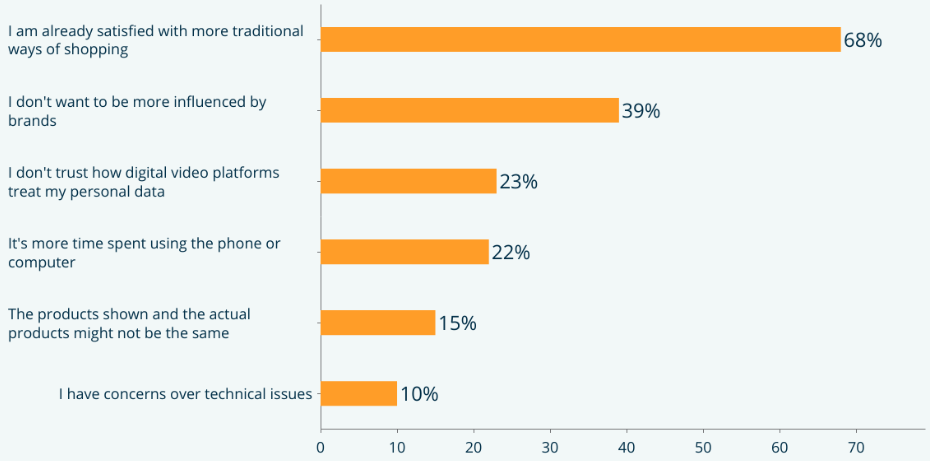
\includegraphics[width=0.8\textwidth]{Images/17.png}
    \caption{2023年Live Commerce and Influencer Survey不喜欢直播购物的原因调研(原问题:“Why are you not interested in using live commerce?”)\cite{21}}
    \label{hate}
\end{figure}

由图(\ref{hate})可以看到,受调研的68\%的人都认为自己已经对传统购物方式十分满意了,并不再需要参与直播促销,他们也不想更多受到品牌效应带来的影响(不过这点值得争议,在中国,品牌效应在直播销售中并没有很强的体现);有人认为这个模式耗时更多;还有13\%的人仍然觉得直播的商品与到手商品可能是不同的,因此更喜欢传统电商方式。

\subsubsection{供应链管理层面}
在供应链管理方面,直播电商和传统电商的运作模式也有差异。直播电商的供应链需要高度灵活,以应对直播活动中快速激增的订单需求。这种即时性促销活动要求商家拥有快速反应的物流体系,以确保在直播结束后能够立即处理大量订单。比如,在中国的双十一购物节期间,许多品牌通过直播产生了数百万订单,这对仓储、物流和供应链的反应能力提出了极高的要求。直播电商链由三个环节组成:一是生产环节,一些厂商将直接成为电商直播,与快递公司合作,减少环节的复杂性,提高销量;二是销售环节,通过直播的方式直接连接原料厂家和消费者,减少传统经销商、经销商、零售商等冗余环节;三是物流环节,与传统供应链相比,减少了从生产到流通环节到最终消费环节的品牌商、经销商、代理商、零售商\cite{22}。

传统电商的供应链管理相对较为稳健,强调的是效率和规模化。平台通过集中化的仓储和标准化的物流流程,实现较低的运营成本和高效的配送体验。以亚马逊为例,其全球范围内的仓储网络和“次日达”服务依赖于成熟的供应链管理,能够在短时间内处理大量订单。这种模式更适合于稳定的、大批量的订单管理,而不是应对突发的高峰需求。

\begin{figure}[htbp!]
    \centering
    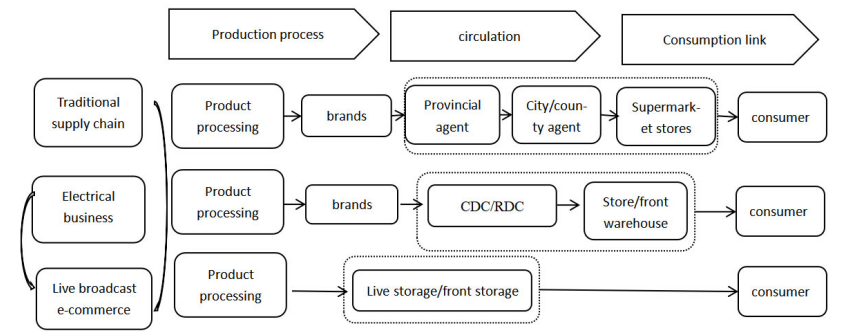
\includegraphics[width=0.9\textwidth]{Images/18.png}
    \caption{传统电商与直播电商供应链流程对比图 \cite{22}}
    \label{diag}
\end{figure}

不过,直播电商供应链的整体概念和本质性质与传统供应链并没有太大的区别,直播电商供应链只是在直播经济发展的驱动下,更加短、快速、高效的集成供应链\cite{22}。


\subsection{直播电商的优势}
直播电商的优势在其成功之处已有所探讨,不妨再看看对消费者和卖家分别的调研结果。

\begin{figure}[htbp!]
    \begin{minipage}[t]{0.457\textwidth}
        \centering
        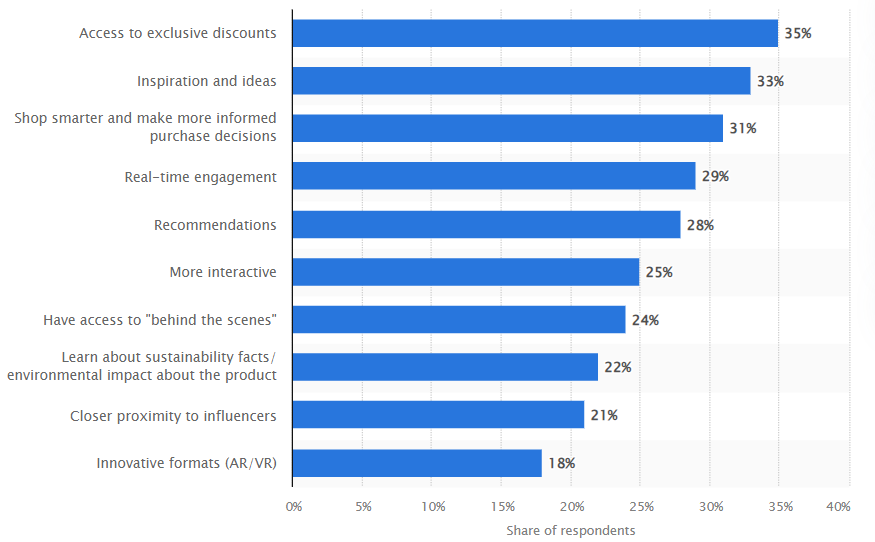
\includegraphics[width=\textwidth]{Images/19.png}
        \caption{2022年全球消费者所感知到的直播购物带来的好处 \cite{23}}
        \label{bene_customer}
    \end{minipage}
    \hfill
    \begin{minipage}[t]{0.53\textwidth}
        \centering
        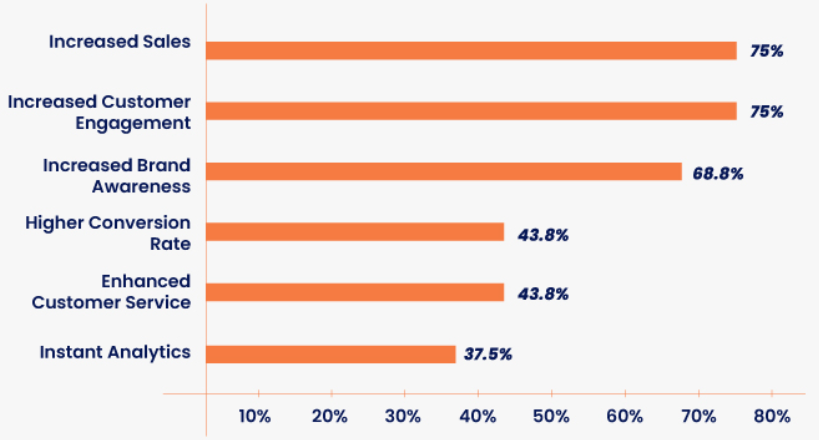
\includegraphics[width=\textwidth]{Images/20.png}
        \caption{2023年全球卖家们所感知到的直播购物带来的好处 \cite{24}}
        \label{bene_seller}
    \end{minipage}
\end{figure}

对于消费者而言,图(\ref{bene_customer})的调查表明,有35\%都认为直播购物让他们享受到了更多的折扣福利,同时提供了灵感,帮助他们做出更明智的购买决策,他们也乐于享受实时互动和个性化推荐。消费者还能通过直播购物了解到产品的幕后信息和可持续性,以及通过创新格式如AR/VR体验更丰富的购物体验。从卖家的角度来看,图(\ref{bene_seller})的数据显示,直播购物能够显著提升销售额和客户参与度,有四分之三的人都这么认为;直播购物还有助于提升他们自己的品牌知名度,增强客户服务,以及提供更深入的数据分析,帮助他们从消费者的视角更好地理解市场和需求。

也就是说,不论是对消费者还是卖家,直播电商的优势都是不言而喻的,这种非单项受益的模式也成为了更好连接卖家和消费者的桥梁,怪不得直播电商如此受青睐!



\subsection{面临的法规和政策挑战}
当然,任何模式都不可能是百分之一百完美的,对于直播电商,也有一些艰巨的挑战。在着重探讨法规和政策方面的挑战之前,不妨先分析一下消费者和卖家受到的挑战。

GoodFirms 在今年的调查报告\cite{24}中与受访者讨论了可能的挑战,先从卖家视角看起。

\begin{figure}[htbp!]
    \centering
    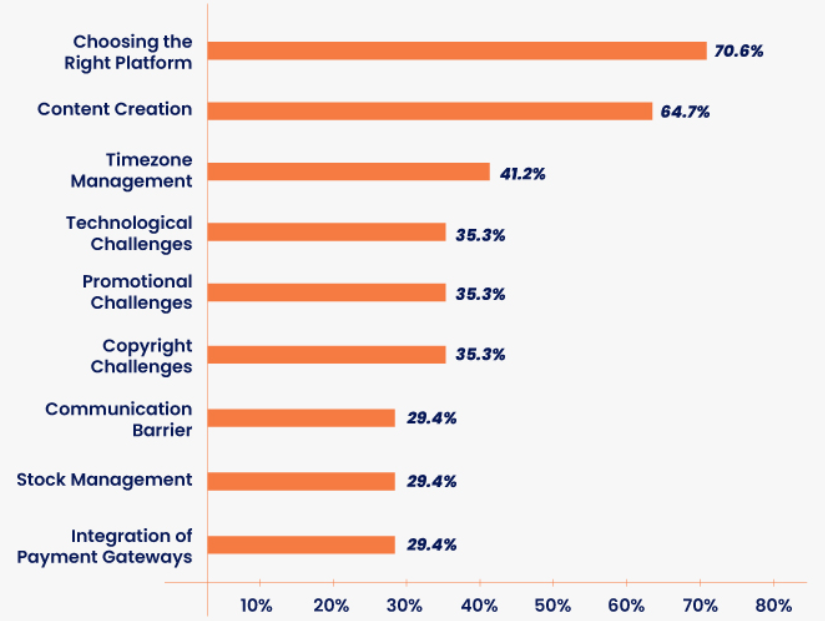
\includegraphics[width=0.7\textwidth]{Images/21.png}
    \caption{2023年卖家在经营直播电商中遇到的问题(原问题:“As a Seller, What are the Challenges of using live-streaming ecommerce?”) \cite{24}}
    \label{challenge}
\end{figure}

如图(\ref{challenge}),70.6\%的卖家认为选择正确的平台是面临的首要问题,这个选择需要与他们的产品和目标市场适配才能发挥很好的效果。内容创作是另一个重大挑战,64.7\%的卖家指出,制作有吸引力且能与观众产生共鸣的内容是困难的。时区的管理则对面向全球市场的卖家是个问题,还有技术挑战、推广和版权问题、沟通障碍(如语言和文化所带来的)和库存管理、支付网关(有研究显示,如果在结账时找不到自己喜欢的付款方式,大约 85\% 的消费者可能终止购物\cite{24}),这一系列复杂的挑战的解决将是他们制胜竞争激烈的直播电商市场的关键。

对于消费者而言,他们面临的挑战则更加直观。\cite{24}的调研显示,71.4\% 的受访者认为技术故障类(如跨国直播网络连接不稳定、直播的突然中断等)干扰会最终会对买家决策产生负面影响;57.1\% 的受访者认为当前直播电商缺乏足够的互动,其中有28.6\% 的人认为他们的疑问在直播购物活动期间并没有得到解决;还有,52.4\%的受访者觉得缺少运输和送货费用的详细信息也是一个大问题,不同于传统电商,有的时候这些信息无法及时获取。

不管怎么说,对于消费者而言,只需“向上滑动”即可购买梦寐以求的商品,直播购物总归相当简单,但主播、卖家和平台来说,在法律法规层面他们需要考虑的就多了。主播可能需要同意平台的使用条款,并可能签署独家协议\cite{25},也就是说,如果我们重新审视一下三者的关系,主播只是卖家或者平台雇佣的“员工”,出于“绩效”考虑,他们在推广商品时自然会带有强烈的个人影响力和广告色彩,也就可能夸大产品效果或隐瞒不利信息,这就可以视为违反广告法了,但是否承担责任是一个法律上的模糊点。在比较严格的情况下,以加拿大为例,Ontario地区的 Consumer Protection Act的法规包括与不公平行为有关的规定,如欺骗性或不合理的陈述、虚假广告等\cite{25}。越来越多的主播获得巨额收入,税务合规问题日益受到重视。一些主播可能未能准确申报收入,导致逃税漏税的风险,是否要对他们设置特别的监管措施呢?这是政府面临的挑战。

卖家呢?卖家需要根据用户行为分析自己的销售效果,一旦涉及到个人信息的数据收集,就与法律脱不了联系了,加拿大的Personal Information Protection and Electronic Documents Act(PIPEDA)规定,企业收集的个人信息必须出于可识别目的并在征得同意的情况下收集,并且只能用于收集个人信息的有限目的,因此卖家必须更加谨慎。

对于平台而言,涉及的面则更广一些。在中国,国家广电总局要求平台对直播内容进行合规性审核,平台需要承担部分监管责任。不仅是卖家,平台也会收集大量用户数据(浏览历史、购物习惯等)欧盟的 General Data Protection Regulation(GDPR)等条规约束平台妥善处理用户数据,否则会面临严重的法律后果。还有一个很重要的问题,跨国平台的推行决定着整个直播电商能否正常运营、市场究竟能拓展到什么程度。就以中国地区为例,这里,直播电商风生水起,相比于美国、欧洲地区许多人对直播购物漠不关心的态度,是一个大好的新兴市场,但是由于法律法规问题,一些大热的直播平台如Twich、论坛Discord、Reddit等无法直接入驻,平台需要适应各个国家不同的规定改变策略,这意味着他们没办法直接使用现有积累了,在与本土平台的竞争中可能会处于劣势。

\subsection{两种模式竞争力SWOT分析}

\begin{figure}[htbp!]
    \centering
    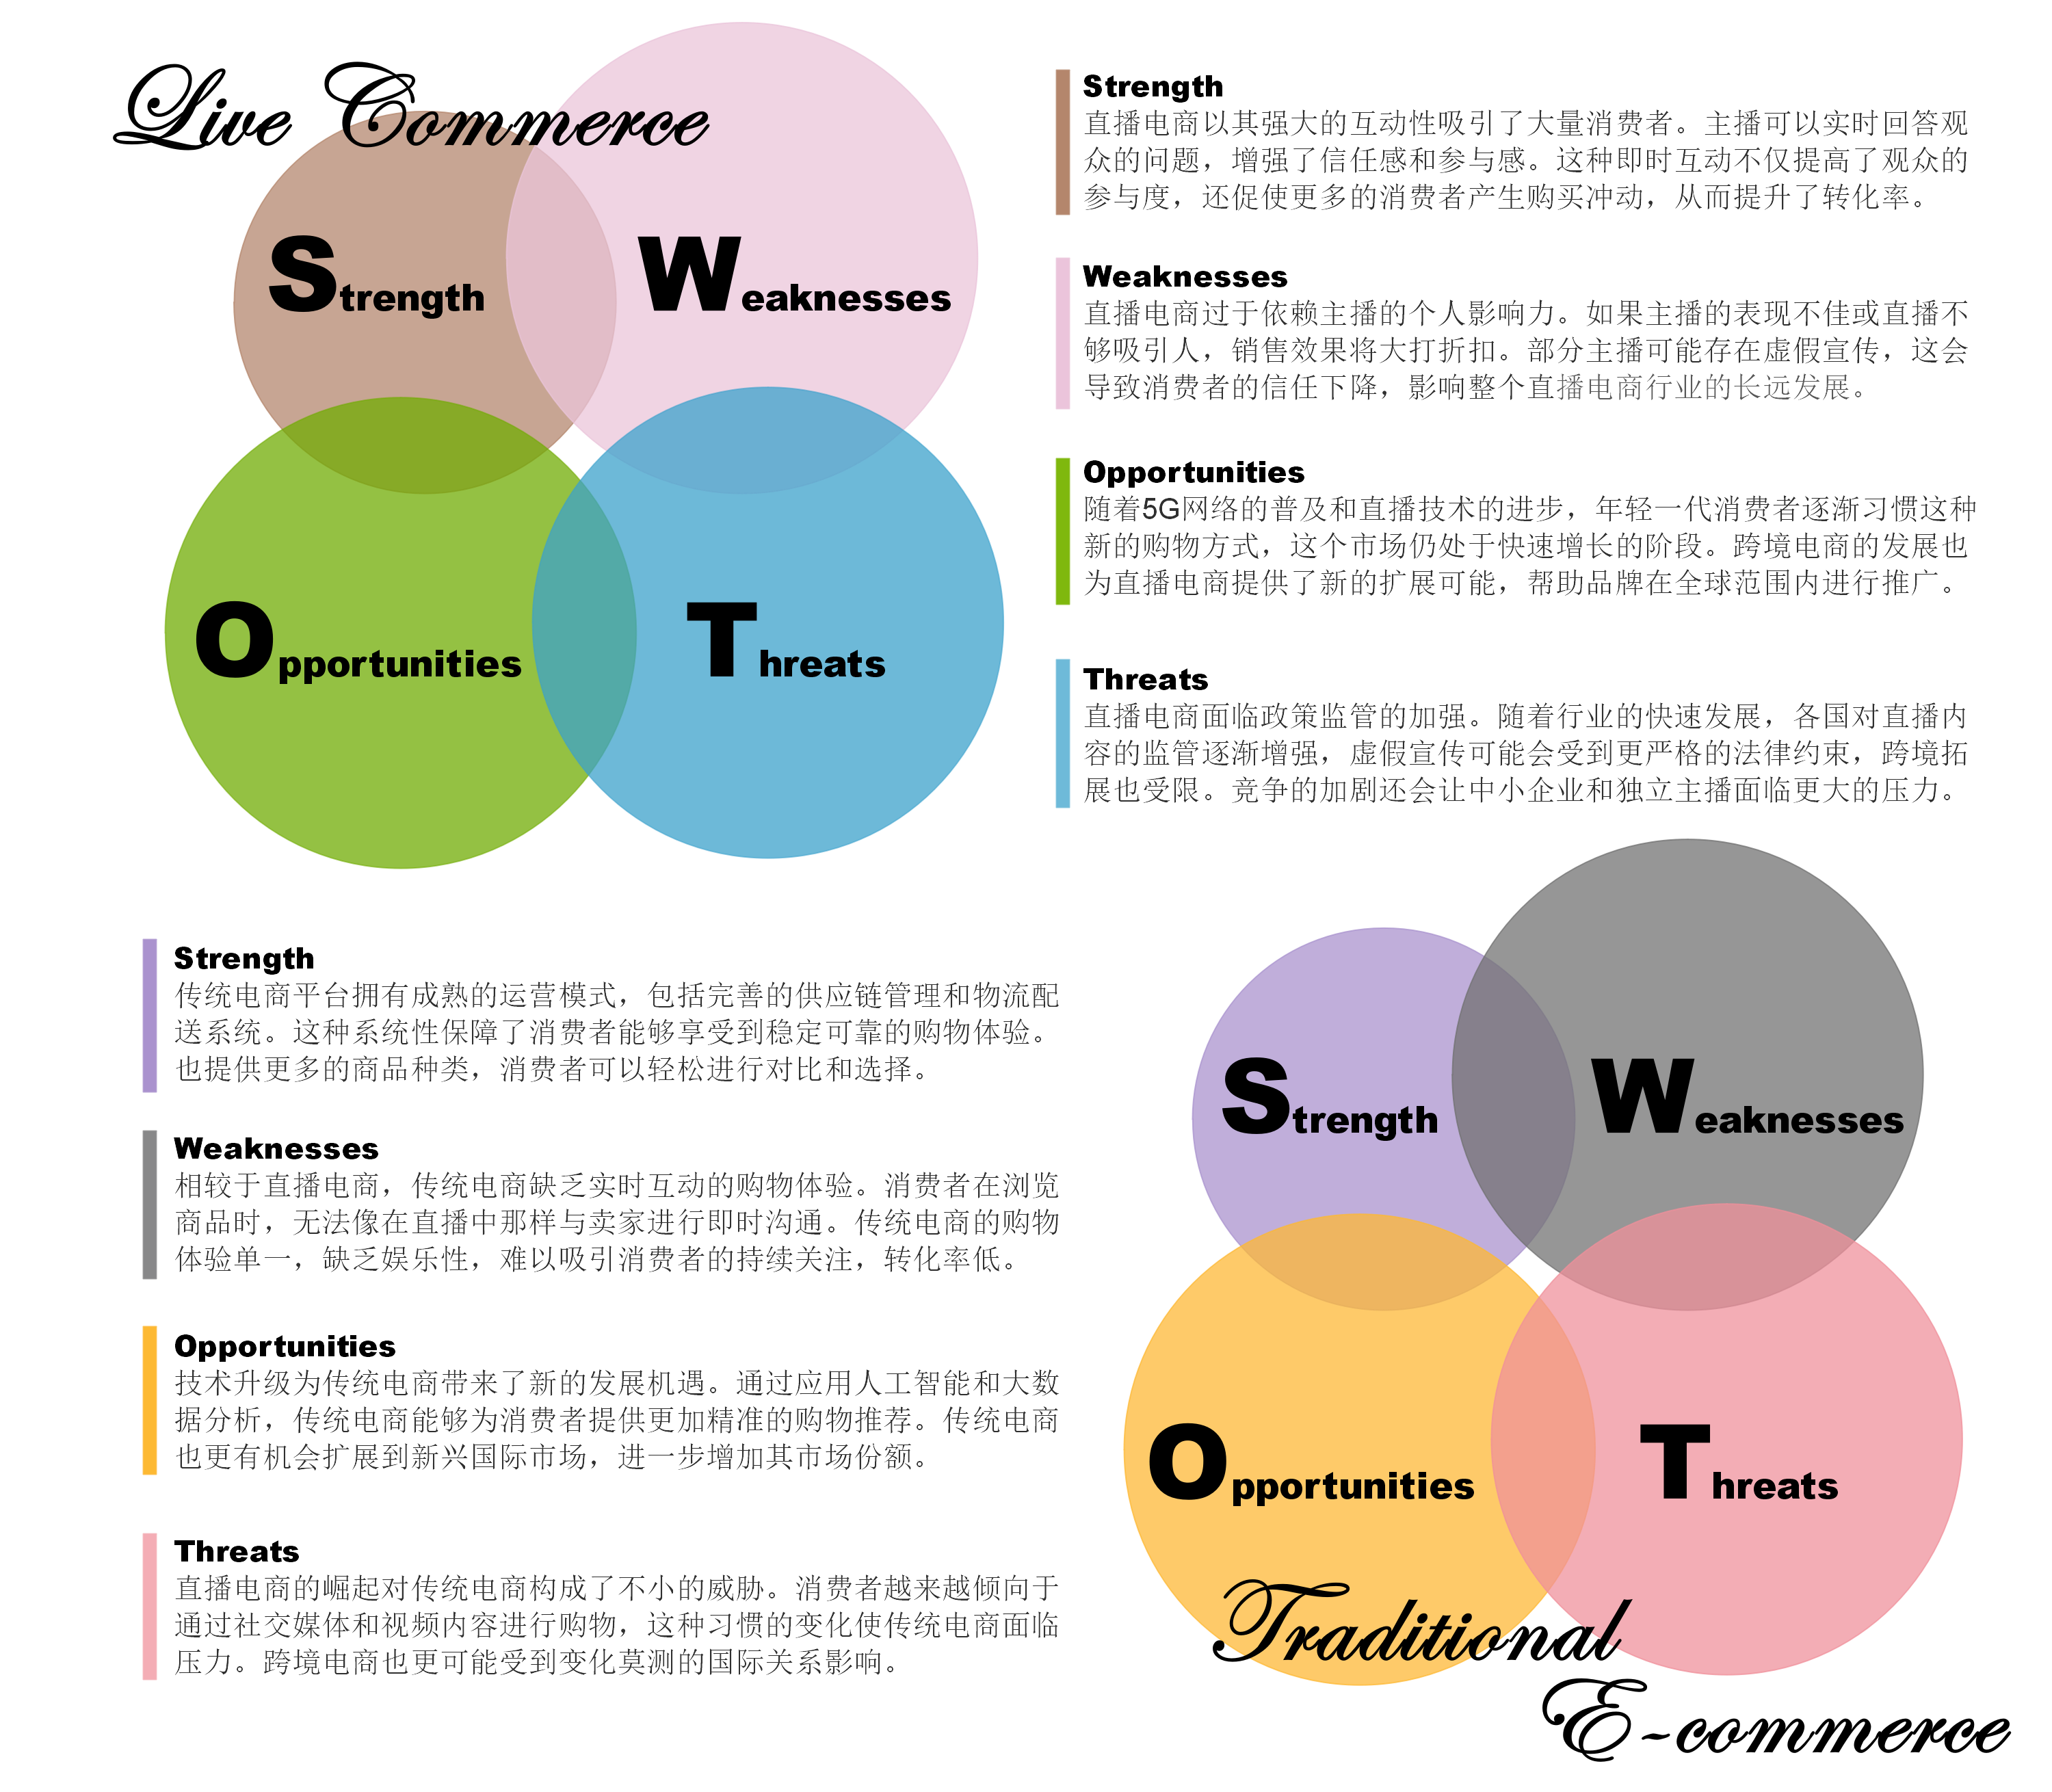
\includegraphics[width=1\textwidth]{Images/22.png}
    \caption{直播电商与传统电商模式的SWOT分析}
    \label{swot}
\end{figure}

从上面的分析来看,由于牵涉到的政治、经济等因素较多,两种模式的客观竞争力可以说是相当的;如果从规模、现状(尤其是鉴于直播电商在美国、欧洲地区不温不火的情况)看来,那么本文作者认为还是传统电商模式更胜一筹;但如果从消费者倾向看来,直播电商确实很不错。

\cite{7}预测,未来医疗保健、工程和金融等领域可能会出现直播电商;小品牌可能选择“纳米网红”(几千粉丝量)推广来节省成本;区块链等技术将用于守护用户的数据和交易的安全性;Metaverse 可能与之集成,引入AR/VR 技术、虚拟主播全天直播等。美好未来还是令人遐想的!
































\newpage
\newgeometry{right=1in,left=1in,top=1in,bottom=0.75in}
\addcontentsline{toc}{section}{参考文献}
\begin{thebibliography}{99}

    \bibitem{1} Vogue Business \& AliExpress. (2024, June 28). \textit{Live streaming ushers in a new era for e-commerce}. Vogue Business. \\ Retrieved October 15, from https://www.voguebusiness.com/story/technology/live-streaming-ushers-in-a-new-era-for-e-commerce

    \bibitem{2} Verified Market Research. (2024, October). \textit{Live e-commerce market by type (domestic, transboundary), application (consumer electronics, furnishing), \& region for 2024-2031 [Graph]}. In \textit{Verified Market Research}. \\ Retrieved October 15, from https://www.verifiedmarketresearch.com/product/live-e-commerce-market/

    \bibitem{3} Market Research Intellect. (2024, October). \textit{Global live e-commerce market size and forecast [Graph]}. In \textit{Market Research Intellect}. \\ Retrieved October 15, from https://www.marketresearchintellect.com/product/global-live-e-commerce-market-size-and-forecast/

    \bibitem{4} Statista. (2024). \textit{Live commerce [Graph]}.  In \textit{Statista}. \\ Retrieved October 16, from  https://www.statista.com/study/105870/live-commerce/ 

    \bibitem{5} Pattern. (n.d.). \textit{We tried out Amazon Live. Here's how it influenced sales}. Pattern.  \\ Retrieved October 16, from https://pattern.com/blog/we-tried-out-amazon-live-heres-how-it-influenced-sales\#:\~:text=\%E2\%80\%8DPro:\%20It's\%20free.,well\%20with\%20low\%\\2Dquality\%20videos.

    \bibitem{6} Cobb, N. (2020, August 19). \textit{Can Amazon Live increase sales? We tested it out}. Pattern.  \\ Retrieved October 16, from https://uk.pattern.com/blog/can-amazon-live-increase-sales-we-tested-it-out/

    \bibitem{7} Goetzen, N. (2021, June 30). \textit{Livestreaming ecommerce takes baby steps in the US}. eMarketer. \\ Retrieved October 16, from https://www.emarketer.com/content/livestreaming-ecommerce-takes-baby-steps-us

    \bibitem{8} Kaziukėnas, J. (2022, January 12). \textit{Amazon Live is embarrassing}. Marketplace Pulse.  \\ Retrieved October 16, from https://www.marketplacepulse.com/articles/amazon-live-is-embarrassing

    \bibitem{9} Korte, B. (2024, January 8). \textit{32 Livestream shopping statistics to know for 2024}. Fit Small Business. \\ Retrieved October 16, from https://fitsmallbusiness.com/livestream-shopping-statistics

    \bibitem{10} Becdach, C., Glaser, D., Sak, N., Wang, K. W.,\& Zimmermann, S. (2023, July 7). \textit{Ready for prime time? The state of live commerce}. McKinsey \& Company. \\ Retrieved October 16, from https://www.mckinsey.com/capabilities/growth-marketing-and-sales/our-insights/ready-for-prime-time-the-state-of-live-commerce

    \bibitem{11} Emplifi. (2024, August 1).  \textit{8 unmistakable benefits of live commerce for you and your customers}. Emplifi. \\ Retrieved October 16, from https://emplifi.io/resources/blog/benefits-of-live-commerce

    \bibitem{12} Bali, N. (2024, April 17). \textit{Content strategies to make live shopping successful for commerce (Updated)}. Channelize. \\ Retrieved October 17, from https://blog.channelize.io/10-content-strategies-to-make-live-streaming-successful-for-commerce

    \bibitem{13} Jenna. (2024, March). \textit{The impact of live commerce on shopping}. Smile.io. \\ Retrieved October 17, from https://blog.smile.io/live-commerce/

    \bibitem{14} Nafea, A. (2024, August 22). \textit{Amazon influencer program: Everything you need to know}. LoudCrowd. \\ Retrieved October 17, from https://loudcrowd.com/blog/amazon-influencer-program-everything-you-need-to-know/
    
    \bibitem{15} Venugopal, A. (2024, January 5). \textit{What is live commerce? A comparison between China and the USA}. ThemeHigh. \\ Retrieved October 17, from https://www.themehigh.com/blog/what-is-live-commerce-a-comparison-between-china-and-the-usa/

    \bibitem{16} Sprii. (2024, June 20). \textit{Live shopping vs. traditional e-commerce: A comparative analysis}. Sprii. \\ Retrieved October 17, from https://sprii.io/articles/live-shopping-vs-traditional\#:\~:text\\=Higher\%20Engagement\%20and\%20Conversion\%20Rates,average\%20for\%20traditional\\\%20e\%2Dcommerce.

    \bibitem{17} Rakuten Insight \& Statista. (2024, September). \textit{Frequency of purchasing through live commerce in Taiwan as of May 2024, by age group [Graph]}. In \textit{Statista}. \\ Retrieved October 17, from https://www.statista.com/statistics/1495963/taiwan-purchase-frequency-in-live-commerce-by-age-group/

    \bibitem{18} Red Stag Fulfillment. (2024). \textit{eCommerce statistics 2024: Trends \& opportunities}. Red Stag Fulfillment.  \\ Retrieved October 17, from https://redstagfulfillment.com/ecommerce-statistics/

    \bibitem{19} Griffith, N. (2024, April 11). \textit{69 mobile commerce statistics (2024)}. SupplyGem. \\ Retrieved October 17, from https://supplygem.com/publications/mobile-commerce-statistics/
    
    \bibitem{20} LocalCircles. (2023, January 11). \textit{7 in 10 Indian online shoppers surveyed believe live commerce will be useful; Want to use it to reach out to someone live for product demo, terms of sale, returns, warranty and pricing [Graph]}. In \textit{LocalCircles}.  \\ Retrieved October 18, from https://www.localcircles.com/a/press/page/live-commerce-standards

    \bibitem{21} Garcia, E. (2023, July 18). \textit{Live shopping: UK SMEs should include discounts and offers in their live stream events [Graph]}. In \textit{Capterra}.  \\ Retrieved October 18, from https://www.capterra.co.uk/blog/4080/uk-consumer-insight-live-shopping

    \bibitem{22} Wang, Y., \& Fang, L. (2021). Research on the supply chain problems and optimization of live streaming e-commerce. \textit{Frontiers in Business, Economics and Management, 2}(3), 100-104. https://doi.org/10.54097/fbem.v2i3.206

    \bibitem{23} Statista. (2022, November). \textit{Perceived benefits of livestream shopping worldwide in 2022 [Graph]}. In \textit{Statista}.  \\ Retrieved October 18, from https://www.statista.com/statistics/1276411/consumers-opinions-on-live-commerce-worldwide/

    \bibitem{24} Sebastian, N. (2024, October 18). \textit{Livestream ecommerce: Market and future scope}. GoodFirms. \\ Retrieved October 18, from https://www.goodfirms.co/resources/livestream-ecommerce-market-future-scope

    \bibitem{25} Monastero, A. (2021, March 29). \textit{The legal considerations of live-stream shopping}. LinkedIn.  \\ Retrieved October 18, from https://www.linkedin.com/pulse/legal-considerations-live-stream-shopping-alessia-monastero/



    
\end{thebibliography}


% \newpage
% \addcontentsline{toc}{section}{Appendix}
% \section*{Appendix} 
% This is Appendix. % 这里写附录



\end{document}
